\documentclass[titlepage]{report}

\usepackage[toc,page]{appendix}
\usepackage{glossaries}
\usepackage{makeidx}
\usepackage{biblatex}
\usepackage{graphicx}
\usepackage{float}

\makeglossaries{}
\loadglsentries{entries}

\makeindex
\addbibresource{bib.bib}

\title{A Peer-to-Peer Content-Sharing Service Built on the Ethereum Blockchain\\\large Extended Abstract}
\author{Sean T. Batzel\\Dr. Bishop}
\date{\today\endgraf\bigskip Submitted in partial fulfillment of the requirements of CMPS/IT 490 --- Computer Projects}

\begin{document}
\maketitle

\nocite{*}

The Ethereum\index{Ethereum} network has attracted a considerable volume of attention in recent months for its native currency, Ether.\cite{ethereum} During the cryptocurrency\index{cryptocurrency} bubble beginning in early 2017 and apparently ending nearly a year later the value of Ether\index{Ether} skyrocketed from just a few dollars to over a thousand dollars. It attracted a staggering number of investors hoping to make a fortune speculating on the value of Ether\index{Ether}, Bitcoin\index{Bitcoin}, and other currencies. Now that the prices have leveled off, the noise has died down somewhat, but is Ethereum's\index{Ethereum} usefulness over? Ethereum\index{Ethereum} itself was never intended as an investment vehicle. Ether was originally conceived of as a way to handle time-sharing on a distributed computing platform. The Ethereum Virtual Machine\index{Ethereum Virtual Machine} itself was designed as a sort of "world computer" which can be used to distribute and run theoretically any program that can be conceived of. People deploying their distributed applications to the EVM\index{Ethereum Virtual Machine} or requesting processing time from one of those applications pay a \gls{gas}\index{gas} fee which sets an upper limit on the amount of time an operation can take on the machine.\cite{yellowpaper} My intention is to build a client/server-analog which uses the Ethereum virtual machine\index{Ethereum Virtual Machine} and \gls{blockchain}\index{blockchain} as the middleware and backend of an email-type service.\\

Since email, instant messaging, and SMS are all commonplace in technology this project may seem to simply reinvent the wheel. These services, though all practical and convenient, tend to be held by a particular group of companies or entities. Content sent between two participants in a conversation are not sent directly from person to person; there must be some intermediary to handle delivery. This project will take advantage of the transaction structure of the blockchain\index{blockchain} and use Ethereum\index{Ethereum} as the delivery and storage system. By committing messages to Ethereum, the ownership and control of the content a party is sending is maintained by the holder of the private keys for the origination of transactions and for the decryption of messages sent to the chain.\\

\begin{figure}[h]
    \centering
    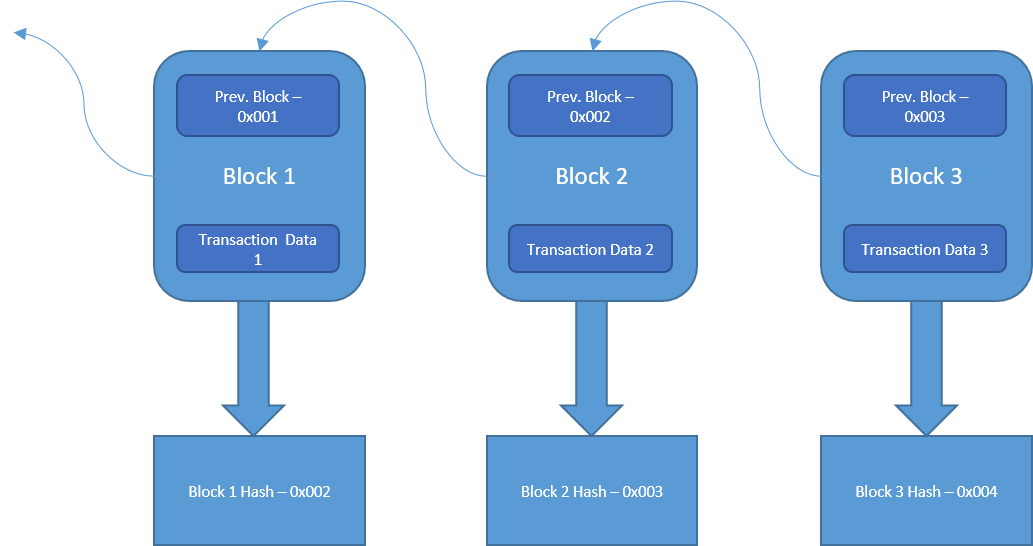
\includegraphics[width=0.5\textwidth]{blockchain}
    \caption{A closer diagram of a general-purpose blockchain. Blocks are connected from one to the next with the capability of adding data payloads to each transaction - in this case, unicode-encoded messages.}
\end{figure}

Consider two conversation partners, Alice and Bob. Bob sends a text message to Alice, which is sent from his device to his carrier. It is relayed through cell towers and data centers, stopping along the way in some unknown number of locations and being saved. Finally it will eventually be delivered, not by the device itself but by the combination of cell carriers, to Alice. There is no promise of security, privacy, or control over the data being sent between endpoints. A message delivery service built on Ethereum\index{Ethereum} would, by nature, circumvent these concerns. Everything occurring on the Ethereum virtual machine\index{Ethereum Virtual Machine} is committed to the blockchain\index{blockchain}. This occurs by distributing every \gls{transaction}\index{transaction} to every computer running a copy of the core Ethereum\index{Ethereum} software. Because every \gls{node} has a copy of that action, it is by definition decentralized. Each transaction is also associated with a pair of public keys (called addresses in cryptocurrency\index{cryptocurrency}), which allows them to prove their origin and destination. As the chain is processed by a number of computers (called miners) tasked with validating and verifying the integrity of the chain\footnote{This is done by using a high-difficulty hashing algorithm to verify that each transaction is a valid extension of the former state of the blockchain\index{blockchain}.}, each \gls{miner}\index{miner} checks to make sure that every one of these transactions, and the metadata associated with them, is completely correct in relation to the rest of the \gls{blockchain}. This allows us to be absolutely certain that every message that this application sends or receives is immutably and provably present.\cite{blockchain}\\

\begin{figure}[h]
    \centering
    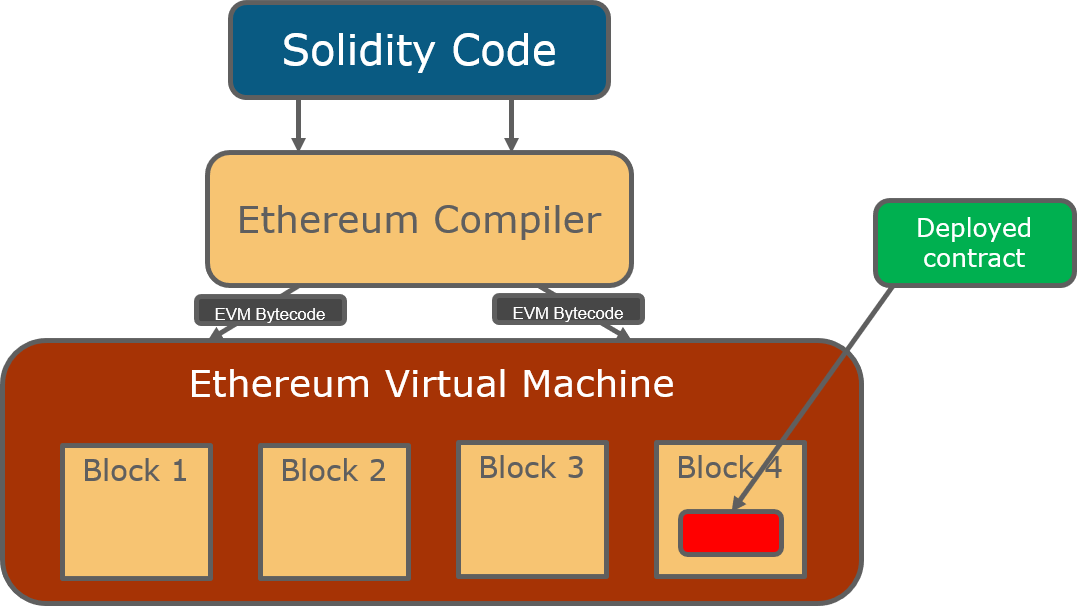
\includegraphics[width=0.5\textwidth]{ethereum}
    \caption{The Ethereum virtual machine functions by distributing bytecode to a number of connected computers, which then execute the given bytecode.}
\end{figure}

On the technical end, this project will ostensibly consist of a database module which will allow us to store content client-side, a cryptographical module using Python's RSA\index{RSA} module, and a blockchain\index{blockchain} module which will allow us to communciate directly with a local version of Ethereum through web3. These functions will all be internal, with a set of functions exposed to the end-user for interacting with the project as a library.\\

I intend for this project to be a proof-of-concept library written in Python\index{Python}. It will require a Python\index{Python} version greater than 3.6, as well as the \gls{web3}\index{web3} implementation for Python\index{Python}.\cite{web3-py} For testing purposes it will also require a \gls{test RPC}\index{test RPC} installed locally in order to test and debug the \gls{smart contract}s\index{smart contract} associated with the application. This smart contract will require a Solidity compiler to be installed in order to produce the compiled bytecode for the contract. In order to maintain the privacy of the messages sent to the blockchain, the library will make direct use of RSA\index{RSA} keypairs to send encrypted messages between users. The test RPC\index{test RPC} I plan on using (Ganache\index{ganache}) will require that the latest version of Node.js\index{Node} installed on the local system. The process of deploying the contract\index{smart contract} and interacting with it will be handled entirely by Python\index{Python} scripts, and in order to deploy the contract\index{smart contract} to the Ethereum\index{Ethereum} \gls{mainnet}\index{mainnet} an RPC pointed at the Ethereum Foundation's official blockchain will be necessary. All of these may be easily installed on most operating systems.\\

Given the time available to me, I am confident that I can implement the core functionality of the client. The database\index{database} and cryptographical\index{cryptographical} modules will be comparatively simple to implement. I am anticipating that the actual process of writing the smart contract\index{smart contract} to handle transaction\index{transaction} processing will be the largest challenge. In terms of goals I would like to reach but which may be more challenging, the current project uses a full local Ethereum\index{Ethereum} node to communicate with the network. The storage requirement for a full node is O(n) where n is the number of transactions\index{transaction} in the blockchain\index{blockchain}. This is impractical for devices with smaller available storage, so the implementation of a \gls{light client}\index{light client} (with storage requirement O(log(n))) integrated into the system would simplify setup and reduce resource usage considerably. I also hope to implement an efficient enough smart contract to optimize the gas usage of the system and thereby retain reasonable transaction fees for users of the service.

\listoffigures
\printindex
\printglossaries{}
\printbibliography{}

\end{document}
